\documentclass[journal,compsoc]{IEEEtran}
\usepackage[UKenglish]{babel}
\usepackage[utf8]{inputenc}

\usepackage{graphicx}
\usepackage{mathtools}
\usepackage{amsmath}
\usepackage{url}
\usepackage{listings}
\usepackage{float}
\usepackage{fancyvrb}
\usepackage{framed}
\usepackage{attrib}
\usepackage{todonotes}

\hyphenation{op-tical net-works semi-conduc-tor}

% Styling commands
\newcommand{\tbf}[1]{\textbf{#1}}
\newcommand{\tit}[1]{\textit{#1}}
\newcommand{\ttt}[1]{\texttt{#1}}

% Document-specific commands
\newcommand{\ws}{WebSocket}
\newcommand{\term}[1]{\tit{#1}}


\begin{document}

\author{\IEEEauthorblockN{Thibault Gérondal, Michaël Heraly}}

\title{Survey paper: \ws}

\date{Tuesday, 27 Oct 2015}

\maketitle
\IEEEpeerreviewmaketitle


%\IEEEdisplaynontitleabstractindextext

\begin{abstract}
The most common way to get information and to communicate through the internet is via the Hypertext Transfer Protocol (HTTP).
Over time, the shared media sent through this communication system has evolved, from text to images and videos.
Interactions between clients and servers have evolved as well.
We went from passive customers who receive information to active clients wanting to communicate in real-time.
The original HTTP was never designed to achieve those needs.
The market found some tricks to bypass these limitations.
However, the HTML5 initiative introduced a real solution to this problem : \ws{}.
This solution brings sockets to the web, so full-duplex communications can be established between clients and servers.
% This paper is only bullshit, but let's try to sell it.

In this survey paper, we describe the older techniques that were used to achieve a full-duplex communication before describing the \ws{} protocol itself.
Then, we explore some experiments that show \ws{} is more efficient than these older methods.
Finally, we discuss the security issues of \ws{}.
\end{abstract}


\section{Introduction}

The Hypertext Transfer Protocol (HTTP) is a stateless request-response protocol in the server-client computing model.
The client submits an HTTP request message and the server provides a response (HTML files, images, etc.).
With the growing popularity of the web, the number of web applications has risen significantly, and the need of interactivity between the client and the server is increasing.
In the original HTTP specifications, interactivity was only possible by loading an entire page in order to upload information to the server or to receive new information from the server.
New features to web browsers have arisen in order to successfully add interactivity without (re)loading pages \cite{RealTimeMonitoringUsingAJAXAndWebSockets}.
Among these, two Javascript API were implemented successively in web \mbox{browsers :} XMLHttpRequest and \ws.


\section{XMLHttpRequest}
\label{XHR}
% Note: real-time interactivity?
One of the first and most used solutions to add real-time interactivity is the XMLHttpRequest (XHR) Object which is a Javascript API that permits the browser to send an HTTP request from a resource to a distant server.
Despite the name of this API, the fetched resource does not have to be an XML file.
In fact, JSON (JavaScript Object Notation) is generally used as it is easier to parse in Javascript \cite{collinalatency}.
This technique is great to send data to the server but not for receiving new data.
If the client wants to keep the information up to date from the server, it will have to poll the server periodically.
This behavior generates a lot of overhead as each request and response will have a full HTTP header and a lot of these requests might return no new data. This technique thus proves to be quite ineffective.

\subsection{The long polling version}

The XHR long polling exploits a loophole inside the \mbox{HTTP/1.1} specifications.
After receiving a HTTP request, a web server is not required to respond immediately, it can defer the reply for a few instants \cite{collinalatency}.
With this technique, the client does not have to poll periodically the server as the web server holds the HTTP request open until it has new data to send to the client, or a timeout expires.
This reduces the amount of useless data transfers and improves the update delay.

\begin{figure}[!ht]
  \centering
  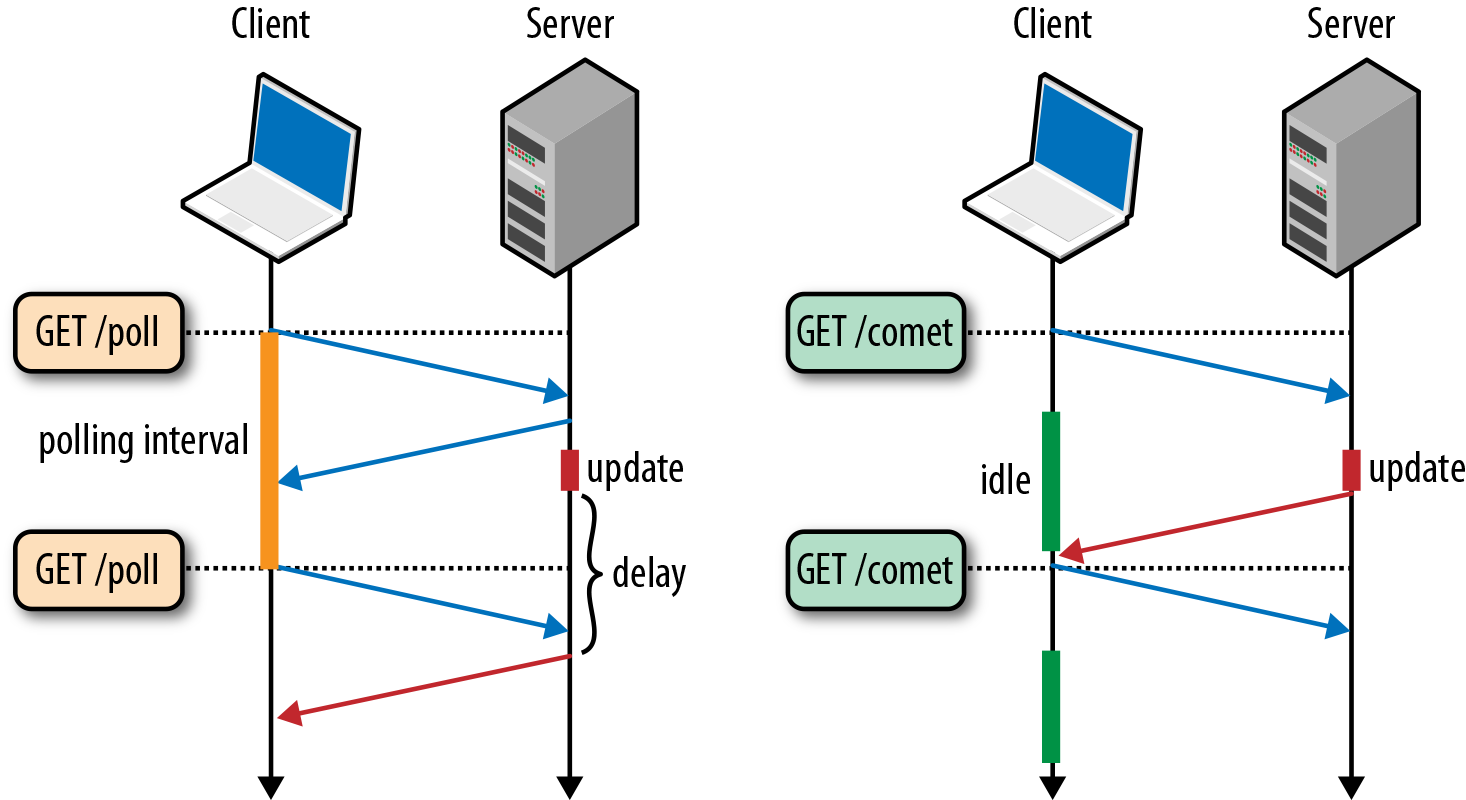
\includegraphics[width=\linewidth]{poll_vs_lpoll}
  \caption{periodic polling (left) versus long polling (right) (from \cite{HighPerfBrowserNetworking:polling})}
  \label{poll_vs_lpoll}
\end{figure}

In Fig.~\ref{poll_vs_lpoll}, on the left, the client periodically polls the server to retrieve updates. This is shown on the figure as the ``polling interval''. When an update occurs on the server side, the client has to wait the next polling to be aware of it. On the right, with long polling, the server keeps the connection open until the update occurs. The periodic polling introduces a delay that long polling can avoid. Also, the first polling of the periodic polling is superfluous as it generates data on the network for no real new input.

\section{\ws{} protocol}
\label{sec:ws}
The \ws{} protocol was standardized by the IETF as RFC 6455 in 2011 \cite{rfc6455}.
This protocol was designed to bring bidirectional, message-oriented streaming of texts and binary data between web browsers and web servers.

As it was designed for the Web, this protocol copes with existing HTTP infrastructure, which means working over HTTP ports 80 and 443.
As the \ws{} protocol is backward compatible with the existing Web infrastructure, it inherits from all its benefits.
First of all, web browsers support the technology natively, including an origin-based security model. % Expliquer dans une section sécurité ?
The Web infrastructure provides URL-based endpoints, which allows to run multiple services on a single TCP port.
It also removes the length limits imposed by plain TCP protocol.
Finally, it allows the traversal of proxies and firewalls.

The \ws{} protocol remains a fully functional protocol that can be used outside the browser.

\subsection{The \ws{} header}
\label{sec:ws-header}
The \ws{} frame structure is shown in Figure \ref{fig:websocket_frame}.

\begin{figure}
    \centering
    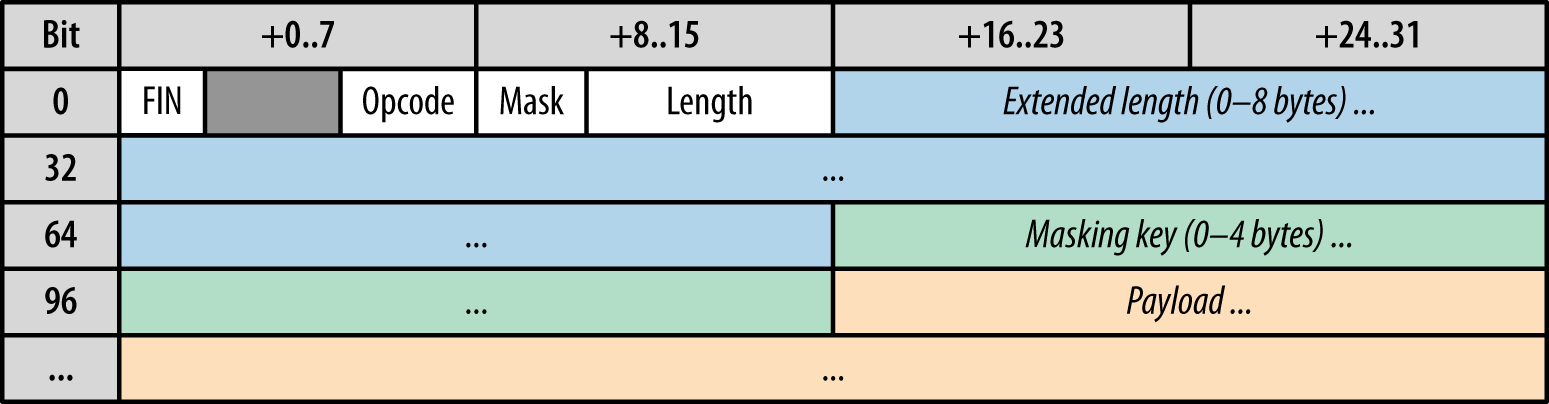
\includegraphics[width=\linewidth]{websocket_frame.png}
    \caption{\ws{} frame structure (from \cite{HighPerfBrowserNetworking:websocket})}
    \label{fig:websocket_frame}
\end{figure}

The \ws{} frame structure is composed of different parts \cite{HighPerfBrowserNetworking:websocket} \cite{performanceEvaluationOfWebsocketProtocol} :
\begin{LaTeXdescription}    % 'description' environment doesn't display well for IEEEtran
    \item[FIN] indicates whether the frame is a final fragment of a message.
    \item[Opcode] indicates the type of the payload data: binary, textual, or protocol-level signaling (e.g. \ttt{close}, \ttt{ping}, \ttt{pong}).
    \item[Mask] indicates whether the payload data is obfuscated (only for messages sent from the client to the server).
    \item[Length] indicates the payload length. If this value is between 0 and 125, this is the actual length.
                    If it is set to 126, the next 2 bytes represent a 16-bit unsigned integer indicating the frame length.
                    If it is set to 127, the next 8 bytes represent a 64-bit unsigned integer indicating the frame length.
    \item[Masking key] is used to disable unwanted payload processed by network intermediaries, like HTTP proxies \cite{performanceEvaluationOfWebsocketProtocol}.
                    This part is omitted in server-originated frames, as the masking is not necessary. See section~\ref{sec:key} for more informations.
    \item[Payload] corresponds to the application data, or custom data if the client and server use a protocol extension.
\end{LaTeXdescription}


%\section{\ws{} Javascript API}
%The \ws{} Javascript API is being standardized by the World Wide Web Consortium (W3C).


\subsection{The \ws{} handshake}
\label{handshake}
The \ws{} protocol is an application-level protocol built on top of TCP \cite{rfc6455}.
It enables bidirectional data transport in Web sessions.
The \ws{} protocol can be used as a Web-based near real-time communication channel.

As the \ws{} is a TCP-based protocol, it needs a TCP connection to be established between the client and the server before any \ws-based interaction can be performed.
As shown on figure \ref{fig:websocket_connection}, the first step is to create a TCP connection, whose handshaking needs three messages between the client and the server (three-way handshake).
At this point, both have access to the plain TCP protocol and they can send application-specific data to each other.
As designed to cope with existing HTTP infrastructure, the client is going to use HTTP to negotiate a switch from regular HTTP to the \ws{} protocol for the rest of the session.
For doing this, the \ws{} protocol is using the \mbox{HTTP/1.1} Upgrade header in the request message.
This header was designed for allowing a client to upgrade from insecure connection to a secure TLS connection.
\ws{} has extended the HTTP Upgrade flow with custom \ws{} headers to perform the negotiation \cite{HighPerfBrowserNetworking:websocket}.
The client also offers a version of the \ws{} protocol to be used.
If the server supports the \ws{} protocol, it replies with an HTTP response with the \ttt{101 Switching Protocols} status code.
From that point, the HTTP-based communication is finished.
The connection can then be used as a two-way communication channel where the client and the server can exchange \ws{} messages.

\begin{figure}
    \centering
    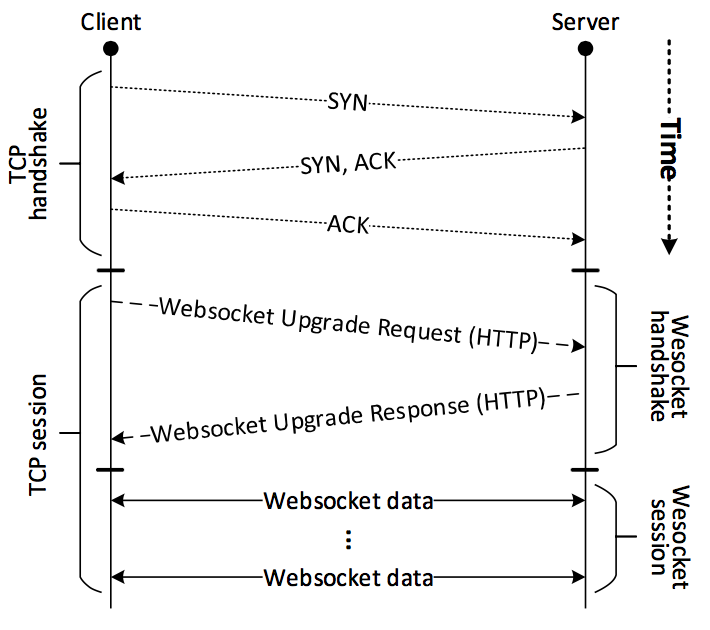
\includegraphics[width=\linewidth]{websocket_tcp_diagram.png}
    \caption{\ws-over-TCP sequence diagram (from \cite{performanceEvaluationOfWebsocketProtocol})}
    \label{fig:websocket_connection}
\end{figure}


\section{Performance of \ws{}}

As we have seen in section~\ref{handshake}, establishing a \ws{} session requires at least five messages.
Making the establishment of a \ws{} connection to take 3.7 times longer than a TCP connection \cite{performanceEvaluationOfWebsocketProtocol}.

As seen in section~\ref{XHR}, XHR and XHR long polling were the two common used methods to simulate a full-duplex connection.
To determine whether \ws{} outperforms these, we are going to inspect the latency and the throughput of each of these techniques.
Plus, we are going to see how good \ws{} is doing compared to TCP.

\subsection{Comparing the latency}

\begin{figure*}[!t]
    \centering
    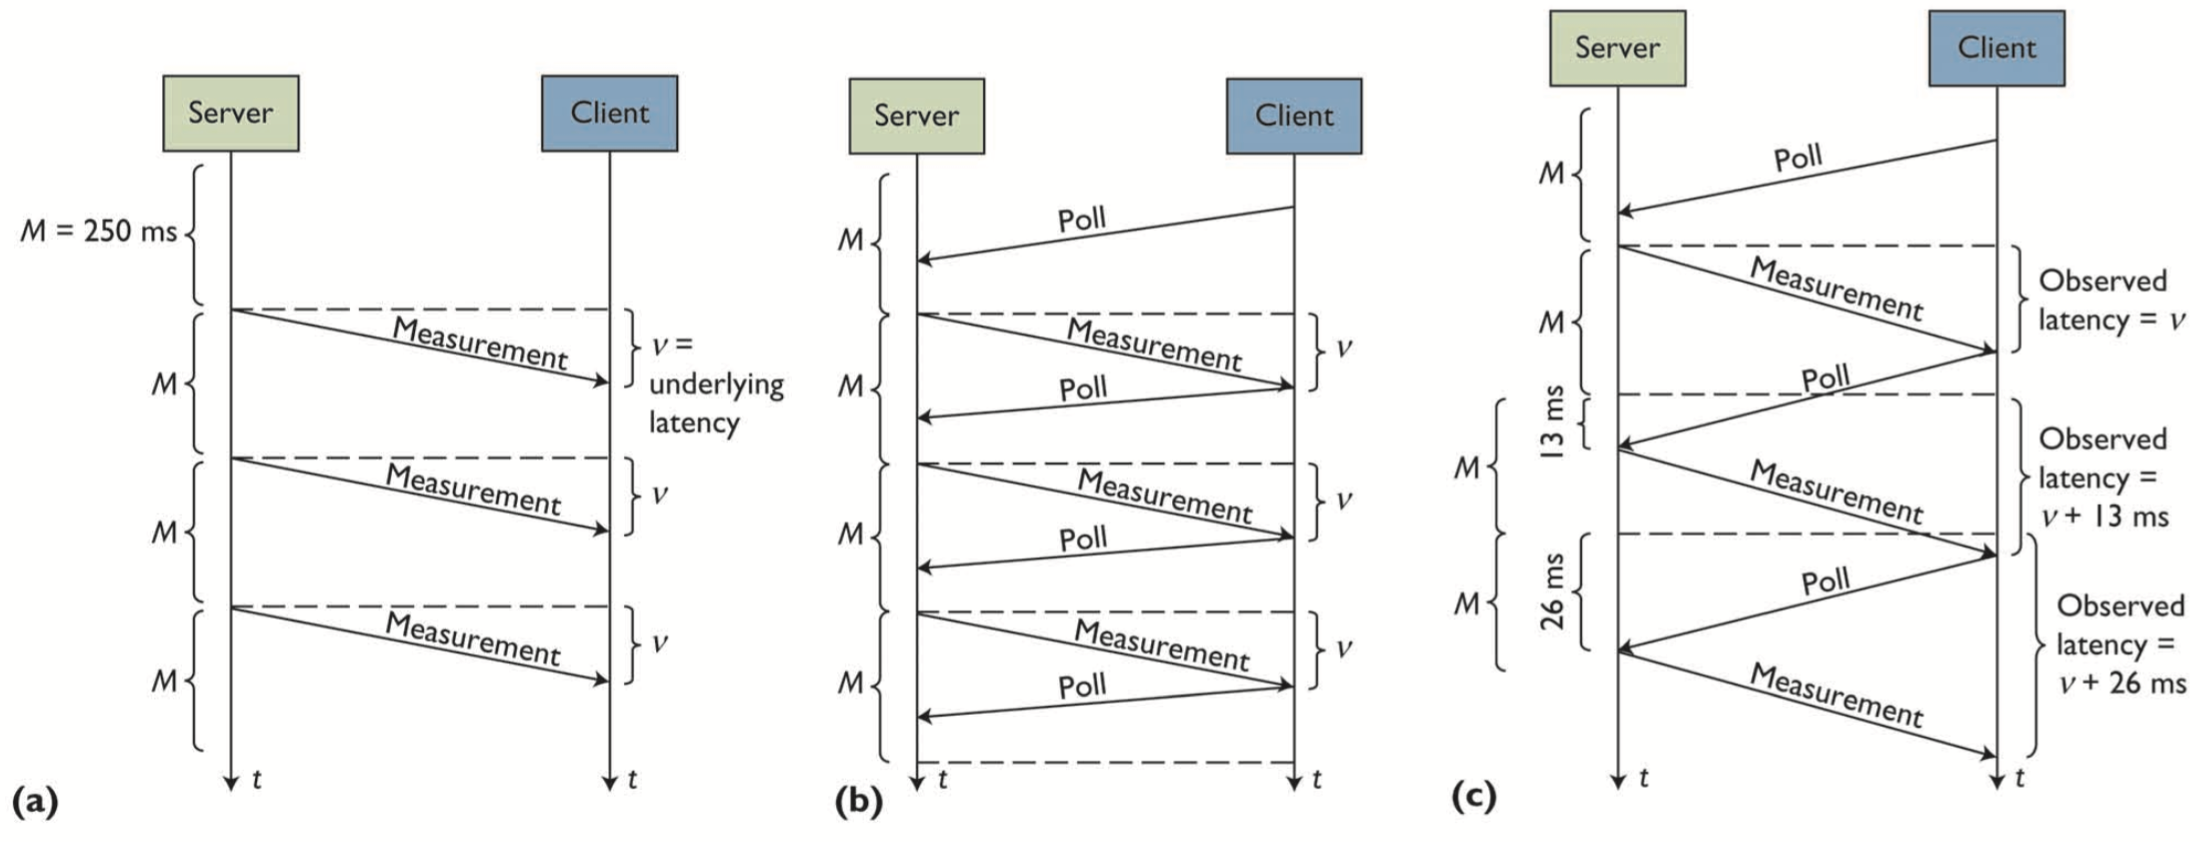
\includegraphics[width=\textwidth]{comdisp.png}
    \caption{Communication behavior in three situations. (a) is using \ws{}; (b) is using long polling with a low underlying latency; (c) is using long polling with a latency greater than half the data measurement rate. Measurements occur at a constant rate of one every $M$ ms. (from \cite{communicationAndDIsplayingRealTimeDataWithWebSocket})}
    \label{fig:comdisp}
\end{figure*}

The experimentation consists of comparing \ws{}, XHR and XHR long polling with different latency in the underlying link.

In \cite{communicationAndDIsplayingRealTimeDataWithWebSocket}, they propose an experiment to measure the latency induced by the use of \ws{} compared to XHR and XHR long polling.
The server receives weather information every 250 ms from a wind sensor and serves it via several ways (WS, XHR and XHR LP).
To compare the latency, clients and server are synchronized.

In this experiment, the XHR without long polling always achieves higher latency.
This is understandable as the client have to periodically poll the server for new data.
The comparison with XHR is not helpful and will not be considered.

Figure~\ref{fig:comdisp}, from \cite{communicationAndDIsplayingRealTimeDataWithWebSocket}, presents three interesting communication behavior.
Figure~\ref{fig:comdisp}a illustrates the \ws{} protocol behavior once it has successfully established the socket connection. Each time the server receives a measurement from the sensor, the server can immediately sends the measurement to the client.
Figure~\ref{fig:comdisp}b illustrates the XHR long polling behavior with an underlying latency low enough ($< 125 $ms, which corresponds to half the $250$ms observation rate) for the client to establish a poll request that the server will keep until it receives new measurement from the sensor.
Figure~\ref{fig:comdisp}c illustrates the XHR long polling behavior with an underlying latency higher than $125$ms.
The client first polls the server, the request arrives at the server before or at exact time a measurement is available.
As a measurement is available, the server sends the sensor message immediately, which closes the connection.
Thus, when the server receives a new poll request from the client, at least one sensor is in the client's queue.
The observed latency is greater than the underlying link.
The long polling is a viable situation as long as the underlying latency is less than half the data measurement rate.
In the situation (a) and (b) of the figure~\ref{fig:comdisp}, the observed latency is the underlying latency.
Meaning that XHR long polling can performs as good as \ws{}.



Another experiment in \cite{collinalatency} is done over a simulated satellite link. They setup a dummy network introducing latency such that the round trip time is fixed at $600$ms.
Then the server or the client have to send 100 messages of 39 bytes. The results are similar.
For \ws{} the mean latency is about $600$ms, the latency of the dummy network. And for the XHR long polling, the mean latency is about $1200$ms, twice the delay introduced.
This makes sense as every time the client (resp. server) has to send (resp. receive) a message in XHR long polling, a new connection has to be established before the data can be issued.
The standard deviation of these values is low.
This is explained by the fact that the whole experiment was conducted on a small network without congestion.

\begin{figure}[!ht]
    \centering
    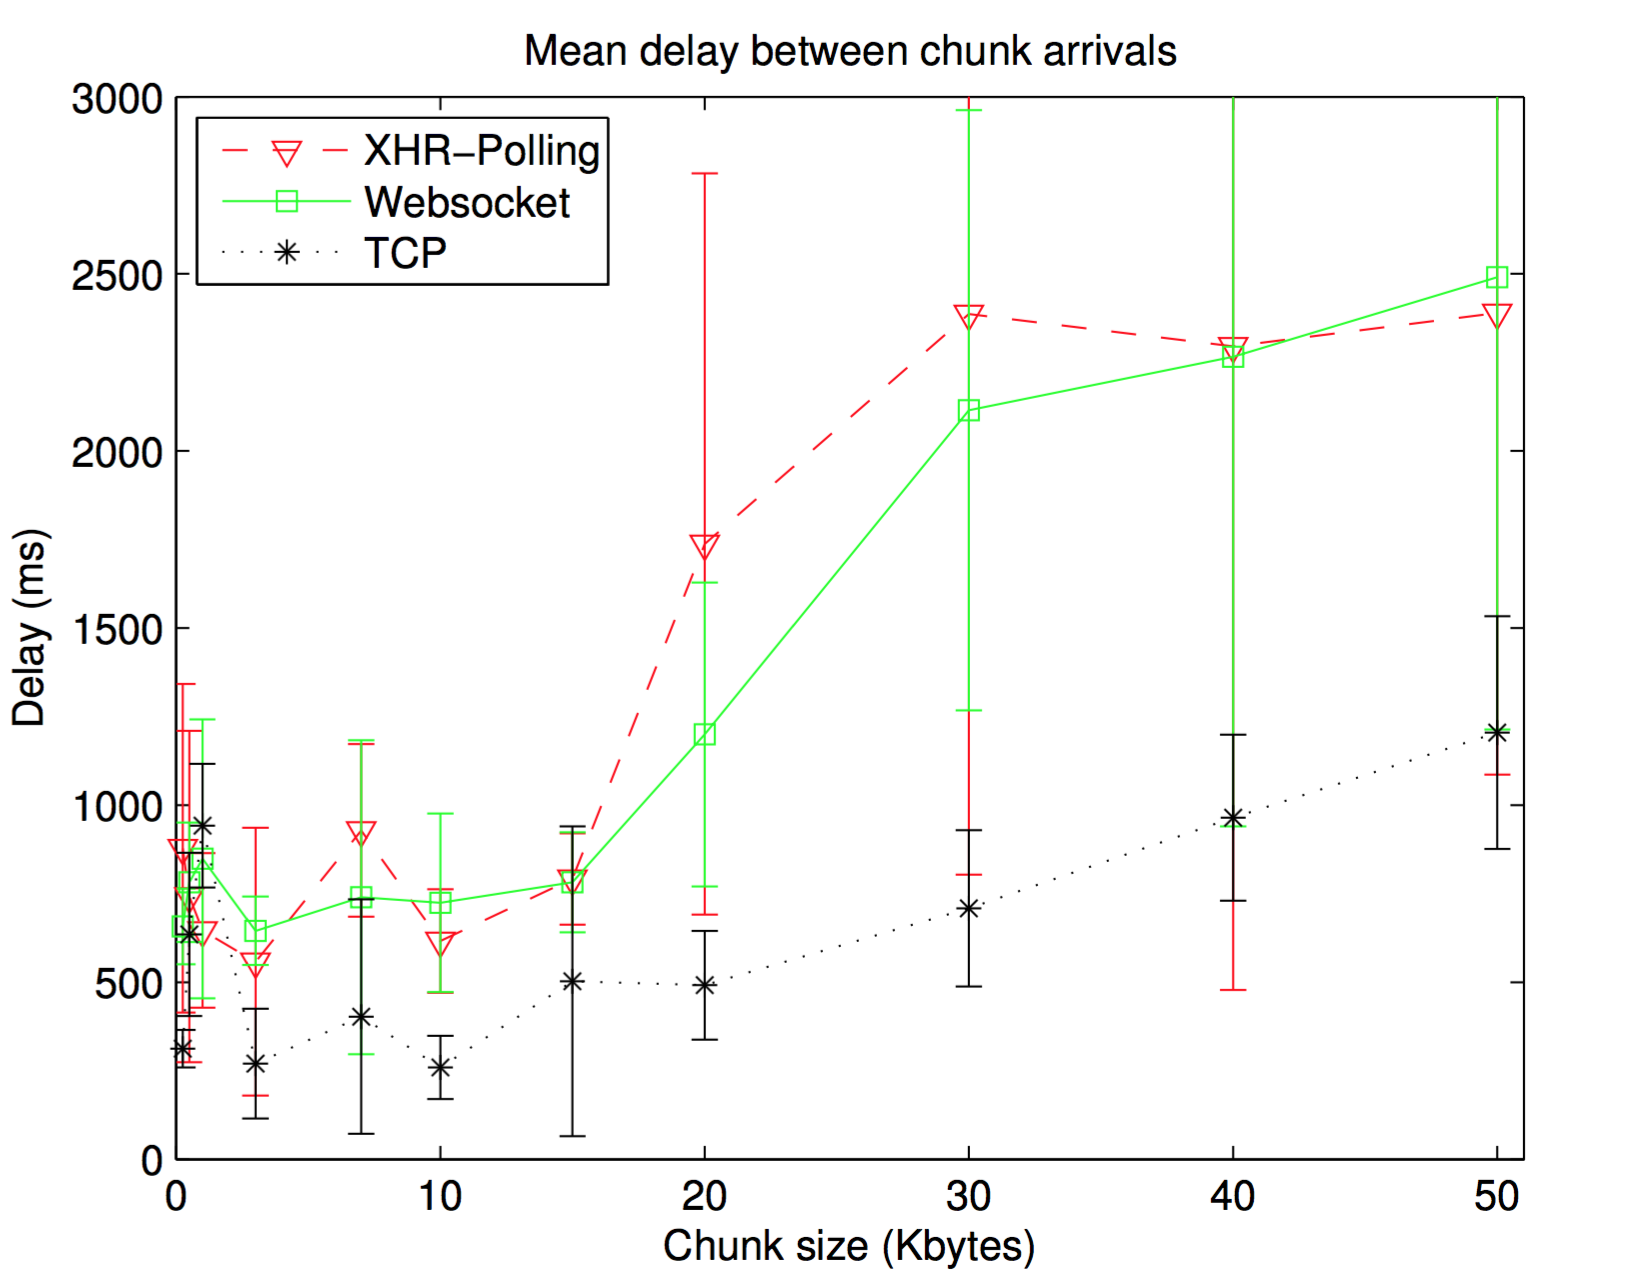
\includegraphics[width=\linewidth]{road.png}
    \caption{Delay over 3G cellular data network (from \cite{roadblock})}
    \label{fig:road}
\end{figure}

These experiments shows that \ws{} achieves better performance than XHR.
But what about \ws{} versus plain TCP ?
This experiment was conducted in \cite{roadblock}.
The setup is a web application that is a simple data echo service.
Clients send a fixed-size chunk of random data to the server that simply sends it back to its respective client.
Figure~\ref{fig:road} shows the average delays in receiving consecutive data chunks as a function of data chunk size.
This experiment is conducted on a 3G cellular data network with three different \mbox{protocols :} XHR long polling, \ws{} and TCP.
We are not going to discuss again the results concerning \ws{} versus XHR long polling.
We can see that what other tests highlighted remain valid in this experiment.
The results of TCP versus \ws{} are questioning.
There is a factor 2-3 increase in delay when using \ws{} as compared to using raw TCP.
Authors of this study conjectured that the reasons for this additional delay are due to additional buffering time at the client, more chatty protocols, and additional overhead.
The first point is mentioned in the IETF HTML5 \ws{} specification ``the implementation MAY delay the actual transmission arbitrarily, e.g., buffering data so as to send fewer IP packets.'' \cite{rfc6455}.
Also, we can notice that the standard deviation is larger for \ws{} compared to TCP.
This standard deviation is called the jitter measurement in networking.
Authors of \cite{roadblock} made another experiment to measure the jitter of each of these protocols.
\begin{figure}[!ht]
    \centering
    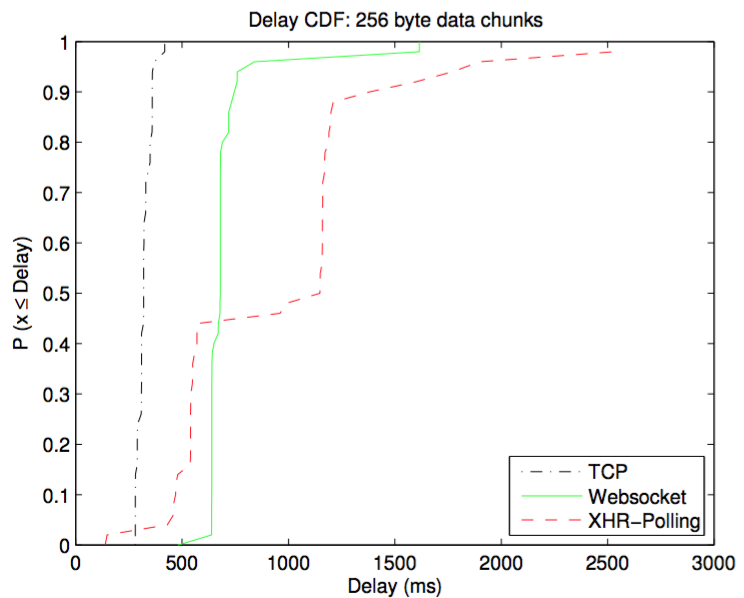
\includegraphics[width=\linewidth]{road_jitter.png}
    \caption{Cumulative distribution function of delays between 256-byte chunk arrivals (from \cite{roadblock})}
    \label{fig:road2}
\end{figure}

For doing this, they measured the delay between successive 256-byte chunk.
The results are shown in figure~\ref{fig:road2}, in a cumulative distribution function.
The figure shows that, with TCP, we can expect that more than 90\% of all data chunks will arrive at the client with an inter-chunk delay of 360ms or less. The corresponding numbers for \ws{} and XHR long polling are $760$ms and $1382$ms respectively.
There is a performance gap between TCP and \ws{} protocol.
This phenomenon is accentuated by the fact that the size of chunk are small.
As the transmission delay is short for small chunks, the main factor of the latency depends on the underlying latency and the processing time of protocols.
To better understand the reason of this gap, we must analyze the generated overhead.

\subsection{Comparing overhead and throughput}

\begin{figure}[!ht]
    \centering
    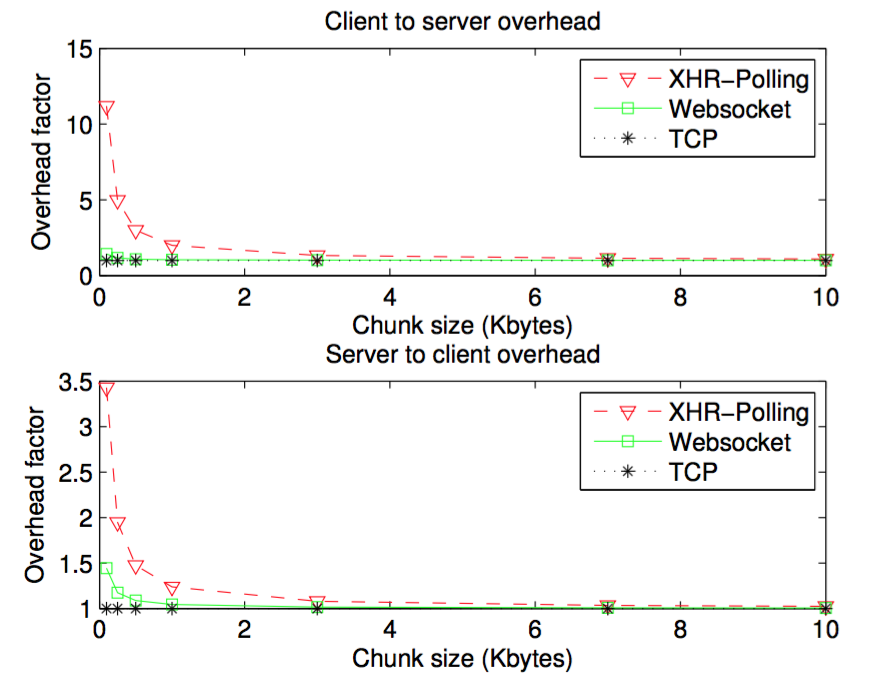
\includegraphics[width=\linewidth]{road4.png}
    \caption{Overhead over a traffic-shaped network (from \cite{roadblock})}
    \label{fig:road4}
\end{figure}

Authors of \cite{roadblock} also studied the throughput of the \ws{} compared to TCP and XHR long polling.
To do so, they used a new setup with a dummy network.
This dummy network will be used to create a traffic-shaped network which restricts total egress \todo{What is egress?} bandwidth to 512kbit/sec and introduces a fixed latency of 50ms.
It will also capture packets to compute the overhead.
The rest of the setup is the same as before, the size of chunk is fixed and the web service is a simple echoing.
In figure~\ref{fig:road4}, they have measured the overhead induced by varying the chunks size.
As we can see, the overhead for XHR long polling is very important.
For small chunk size, it can be up to ten times the size of the data.
This is easy to understand as XHR uses HTTP.
Thus, the HTTP header is included in each request and response in XHR long polling.
And the HTTP header size is unpredictable as it contains a lot of superfluous informations in our case, such as browser cookies.
It explains why the overhead from the client to the server is more important than the overhead from the server to the client as the client is more likely to add unnecessary header.
We can see that the overhead factor for \ws{} is more reasonable.
This overhead is due to the header of the \ws{} protocol described in section~\ref{sec:ws-header}.
For a chunk of 256-byte transmitted from the client to the server, the XHR long polling imposes a large overhead factor of up to 5.
When the overhead factor of \ws{} is at 1.16.


\begin{figure}[!ht]
    \centering
    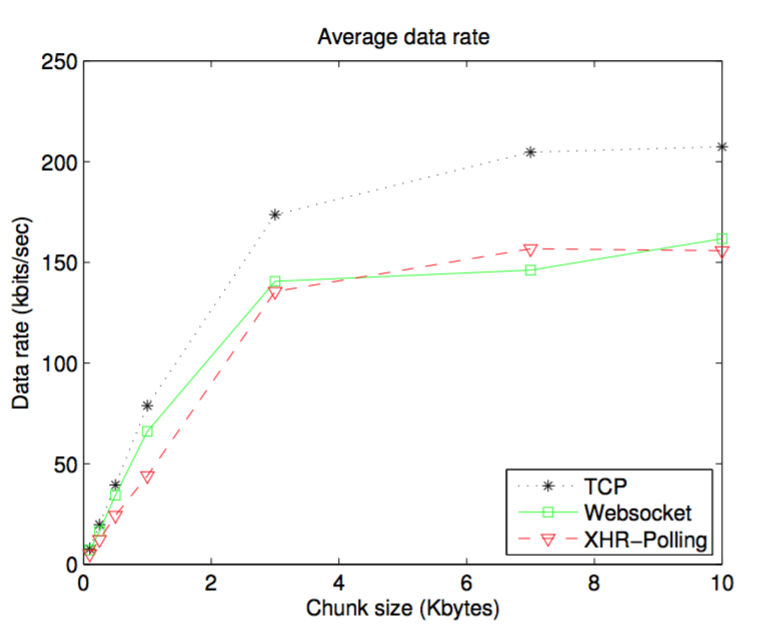
\includegraphics[width=\linewidth]{road3.png}
    \caption{Throughput (from \cite{roadblock})}
    \label{fig:road3}
\end{figure}

Authors of \cite{roadblock} also studied the throughput of the \ws{} compared to TCP and XHR long polling.
To do so, they used the same setup as described before (traffic-shaped network).
The figure~\ref{fig:road3} shows the net throughput (amount of useful data received, stripped of protocol overhead, in kbits/s) at the client as a function of data chunk sizes.
We can see that TCP performs better throughput than \ws{} and XHR long polling.
For a 1kB chunks, TCP achieves a throughput of 78kbits/s as compared to 66kbits and 44 kbits/s in the case of \ws{} and XHR long polling respectively.
We know that the throughput is dependent of the round trip time and the overhead, so these results are not surprising.

In \cite{EV}, authors also analyzed the performance of \ws{} throughput for electric vehicles communicating with \ws{}.
They have created an Android application simulating an electric vehicle.
The application uses the 3G cellular data network to communicate with a server.
They conclude that \ws{} is inefficient in comparison to regular TCP as TCP requires 40\%-50\% less bit rate than \ws{} for their messages.
The size of status message of their electric vehicles is about 500 bytes.
As the message is shorter, the overhead ratio is higher.
These results are in agreement with the previous ones.
The authors highlight the fact that \ws{} can need \ttt{keep-alive} traffic to keep the connection open.
The \ttt{keep-alive} can spend a lot of superfluous traffic, especially if the exchanged messages are small.

%To reduce network utilization, they invented three methods in order to aggregate the %data.
%The first is time sampling, every T second, the EV sends informations.
%The second is distance sampling, every D meters, the EV sends informations.
%And the last one is the bundling.
%The data are sent in bundle.
%These three parameters are represented as a tuple (T,D,B).
%For instance, (0, 0, 1) means that there is no periodic and distance sampling and B=1 means that there is no bundling as the bundle contains only one sample.

\section{Security}

As said in section~\ref{sec:ws}, \ws{} benefits from security model of the HTTP but also inherits problems thereby.

\subsection{Same origin security}

During the handshake, the browser adds the \ttt{Origin} header to the HTTP Upgrade request.
The server can accept or deny the request based on this header.
Also, even if the origin is not the same, it is possible to establish a connection thanks to the Cross Origin Request Sharing (CORS) \cite{talkingtoyourself}.
The principle is the same as in HTTP.

\subsection{Proxies and black boxes}
\label{sec:key}
As the web is the most common way to communicate on internet, there are a lot of proxies and black boxes that intercept the traffic going through port 80.
Theses intermediaries might not understand what happens once the negotiation for \ws{} Upgrade is achieved.
And this can be problematic.
When a proxy or black box does not understand what happened, the traffic can be altered or discarded.
This will make the \ws{} communication unusable.
This poses a problem for the progress of the adoption of the \ws s.

But the most undesired behavior was that a proxy bufferised the \ws{} frames.
As described in \cite{talkingtoyourself}, if a proxy is doing such a thing, an attacker can poison the cache of the proxy with malicious payload.
When a legitimate user behind the proxy wants to retrieve the \ws{}, he will get the malicious payload from the poisoned proxy's cache.
To counter this, a masking key is sent by the client, this key will be used by the server to mask the payload (masking key XOR payload).
As the client knows the masking key, it can decode the payload and be sure that the payload wasn't modified by any proxies or black boxes.
This mechanism defeats the cache poisoning attack.

\subsection{TLS}
\ws{} supports TLS.
This is useful to cipher payload but not only.
As proxies and black boxes can do nothing with TLS communication, by ensuring that a website is using secure \ws{}, it also ensures that no proxy or black box will prevent the connection.


\section{Conclusion}
In this paper, we covered the different solutions that were used prior to the \ws{}.
These include XHR polling and XHR long-polling.
Then, we introduced the \ws{}, which is composed by the \ws{} JavaScript API and the underlying \ws{} protocol.
We saw that the \ws{} protocol was based on TCP.
We presented how two hosts could connect to each other to create a \ws{} session.
We also exposed the \ws{} header to explain the \ws{} frame structure.
We ended the paper by comparing the technology with the prior solutions, with a focus on the throughput and the latency.
It turns out that the \ws{} causes lower performance compared to the plain TCP protocol.
It causes some overhead and has a higher latency than a plain TCP connection.
However, it is still better than the alternative solutions, as XHR polling and XHR long-polling.
The overhead caused by the \ws{} is negligible for practical use, and for situations where a lot of data are sent between the client and the server, the cost of the initial HTTP handshaking is amortized by the large number of payload transfers.

% Rajouter une conclusion sur les quelques points de sécurité abordés
\todo{Talk about security}

Finally, the \ws{} protocol is a useful addition to the Web, which brings a full-duplex communication that is more efficient than the other solutions which try to simulate an equivalent behavior in HTTP-based applications.

\ifCLASSOPTIONcaptionsoff
  \newpage
\fi


\bibliographystyle{IEEEtran}
\bibliography{bibi}


\end{document}
